\documentclass[a4paper,12pt,oneside]{article}
\usepackage[portuguese]{babel}
%\usepackage[latin1]{inputenc}
\usepackage[utf8]{inputenc}
\usepackage[T1]{fontenc}
\usepackage{fancyhdr}
\usepackage{pdfpages} 
\usepackage{mdwlist}
\usepackage{bm}
\usepackage{blindtext}
\usepackage{array}
\usepackage{multicol}
\usepackage{multirow}
\usepackage{mdwlist}
\usepackage{enumitem}
\usepackage[numbers]{natbib}
\usepackage{url} 
\usepackage{graphicx}
\usepackage{caption}    
\usepackage{amsmath}
\usepackage{amsthm}
\usepackage{amsfonts}
\usepackage{mathrsfs}
\usepackage{amssymb}
\usepackage{mdframed}
\usepackage{xcolor}
\usepackage{fourier-orns}
\usepackage{geometry}
\usepackage{parskip}
\usepackage{listings}
\usepackage{setspace}
\usepackage{imakeidx}
\usepackage{makeidx}
\usepackage{authblk} 
\usepackage{setspace} 
\usepackage{etoolbox}
\usepackage[
            pdftex
            ,plainpages=false
            ,pdfpagelabels
            ,pagebackref = false
            ,hyperindex
            ,breaklinks=true 
            ,colorlinks=true 
            ,citecolor=black 
            ,linkcolor=black
            ,urlcolor=black
            ,filecolor=black
            ,bookmarksopen=true
            ]{hyperref}
%%%%%%%%%%%%%%%%%%%%%%%%%%%%%%%%%%%%%%%%%%%%%%%%%%%%%%%%%%%%%%%%%%%%%%%
\makeatletter
\renewenvironment{abstract}{
    \if@twocolumn
        \section*{Abstract}
    \else
        \small
        \begin{center}
            {\bfseries \abstractname\vspace{-.5em}\vspace{\z@}}%
        \end{center}
        \noindent
    \fi
}
%{\par\vspace{1.5em}\noindent\hrulefill\par} 
\makeatother
%%%%%%%%%%%%%%%%%%%%%%%%%%%%%%%%%%%%%%%%%%%%%%%%%%%%%%%%%%%%%%%%%%%%%%%
\lstset{
  language=Python,
	basicstyle = \fontsize{10}{12}\ttfamily%\small
  keywordstyle=\color{blue},
  commentstyle=\color{green!60!black},
  stringstyle=\color{red},
  showstringspaces=false,
  breaklines=true,
  frame=single,
  numbers=left,
  numberstyle=\tiny\color{gray},
  captionpos=b,
  escapeinside={(*@}{@*)} % If you need to include LaTeX within your code
}
%%%%%%%%%%%%%%%%%%%%%%%%%%%%%%%%%%%%%%%%%%%%%%%%%%%%%%%%%%%%%%%%%%%%%%%
\textheight 9in  
\topmargin -.5in   
\def\baselinestretch{1.06}
\textwidth 6.6in 
\oddsidemargin 0in 
\evensidemargin 0in
\geometry{left=25mm,right=25mm,top=25mm,bottom=25mm}
\addtocontents{toc}{\protect\setcounter{tocdepth}{2}}
\numberwithin{equation}{section}
%%%%%%%%%%%%%%%%%%%%%%%%%%%%%%%%%%%%%%%%%%%%%%%%%%%%%%%%%%%%%%%%%%%%%%%%%%%%
\lstset{
  language=Python,
	basicstyle = \fontsize{10}{12}\ttfamily%\small
  keywordstyle=\color{blue},
  commentstyle=\color{green!60!black},
  stringstyle=\color{red},
  showstringspaces=false,
  breaklines=true,
  frame=single,
  numbers=left,
  numberstyle=\tiny\color{gray},
  captionpos=b,
  escapeinside={(*@}{@*)} % If you need to include LaTeX within your code
}
%%%%%%%%%%%%%%%%%%%%%%%%%%%%%%%%%%%%%%%%%%%%%%%%%%%%%%%%%%%%%%
\DeclareMathOperator{\sech}{sech}
\newcommand{\sen}{\mathrm{sen}}
\newcommand{\dd}{\mathrm{d}}
\newcommand{\keywords}[1]{\textbf{\textit{keywords:}} #1}
\newcommand{\palavraschave}[1]{\textbf{\textit{palavras-chave:}} #1}
\newcommand{\EE}{\mathbf{e}}
\newcommand{\RR}{\mathrm{R}}
\newcommand{\GG}{\mathbf{G}}
\newcommand{\TT}{\mathrm{T}}

\def\be{\begin{equation}}
\def\ee{\end{equation}}
\def\ni{\noindent}

\addtocontents{toc}{\protect\setcounter{tocdepth}{2}}
\numberwithin{equation}{section}
\setlength{\parindent}{1cm}

\def\NAT@def@citea{\def\@citea{\NAT@separator}}%
%%%%%%%%%%%%%%%%%%%%%%%%%%%%%%%%%%%%%%%%%%%%%%%%%%%%%%%%%%%%%%%%%%%%%%%%%%%%
% Number exercises within subsections
\newtheorem{exercise}{Exercise}[section]
\newtheorem{definition}{Definition}
\newtheorem{example}{Example}
\newtheorem{corollary}{Corollary}

%%%%%%%%%%%%%%%%%%%%%%%%%%%%%%%%%%%%%%%%%%%%%%%%%%%%%%%%%%%%%%%%%%%%%%%%%%%%
\makeindex

\title{Um problema de matemática recreativa em geometria plana sobre comprimentos de arco em cadeias de círculos tangentes}

\author[1]{Osvaldo L. Santos-Pereira 
\thanks{olsp@if.ufrj.br}
\thanks{\href{https://orcid.org/0000-0003-2231-517X}{ORCID: 0000-0003-2231-517X}}}
\affil[1]{Programa de Pós-Graduação Multidisciplinar em Física Aplicada, Instituto de Física, Universidade Federal do Rio de Janeiro}
\date{\today}

\begin{document}
\maketitle

\begin{abstract}
\ni
Este texto apresenta uma solução para um problema de geometria plana e sua generalização. O problema foi retirado do Volume 9 da coleção \textit{Fundamentos da Matemática Elementar}, uma clássica coleção brasileira de livros de matemática elementar voltada a estudantes do ensino médio, composta por 11 volumes. O Volume 9 é dedicado à geometria plana e contém diversos problemas que, apesar de sua formulação elementar, oferecem valiosas oportunidades para o desenvolvimento do raciocínio matemático.
\end{abstract}

\noindent\textbf{Palavras-chave:} matemática recreativa; geometria plana; circunferências tangentes; arcos circulares; comprimento de arco; ângulo explementar


\section{Introdução}

A geometria plana euclidiana é um dos temas mais adequados ao desenvolvimento do raciocínio matemático, especialmente para estudantes em estágios iniciais de formação. Seus objetos são visualmente intuitivos; no entanto, suas conclusões exigem definições precisas, organização lógica e demonstrações rigorosas. Nesse contexto, os estudantes são naturalmente levados a distinguir entre o que parece verdadeiro em uma figura e o que pode ser demonstrado com base em axiomas, teoremas e resultados previamente estabelecidos. Problemas envolvendo retas, ângulos, circunferências, polígonos, tangência e congruência oferecem um ambiente fértil para a prática de técnicas de demonstração, tais como demonstração direta, demonstração por contradição, construções auxiliares, decomposição de figuras e generalização a partir de configurações particulares. Por essa razão, a geometria plana ocupa uma posição privilegiada na educação matemática: ela conecta a intuição visual ao raciocínio dedutivo, mostrando que a matemática não consiste meramente no cálculo de respostas numéricas, mas na construção disciplinada de argumentos.

O problema analisado aqui diz respeito ao comprimento de uma curva formada por arcos sucessivos de circunferências tangentes entre si. Ele foi retirado do Problema 737 do Volume 9 da coleção \textit{Fundamentos da Matemática Elementar}, na edição utilizada como referência neste trabalho. Como se trata de uma edição mais antiga do livro, o mesmo problema pode não aparecer com a mesma numeração, ou pode até mesmo não aparecer, em edições mais recentes.

Embora o cálculo seja simples, o exercício ilustra uma característica importante do pensamento matemático: a capacidade de identificar a estrutura geométrica subjacente a uma configuração particular e, em seguida, generalizar o resultado a uma configuração arbitrária. Nesse sentido, o problema pertence naturalmente à matemática recreativa, na qual problemas elementares servem como porta de entrada para a abstração, o reconhecimento de padrões e a generalização. O enunciado do problema é o seguinte. A Fig.,\ref{fig:geometric-configuration} também faz parte do enunciado.

\ni
\textbf{Problema.} \textit{Se os ângulos nos vértices $O_1, O_2, O_3, O_4$ e $O_5$ medem, respectivamente, $90^\circ$, $72^\circ$, $135^\circ$, $120^\circ$ e $105^\circ$, e os raios das circunferências centradas nesses vértices medem, respectivamente, $18,\mathrm{cm}$, $35,\mathrm{cm}$, $24,\mathrm{cm}$, $36,\mathrm{cm}$ e $48,\mathrm{cm}$, determine o comprimento da curva $AB$.}


\begin{figure}[ht]
\centering
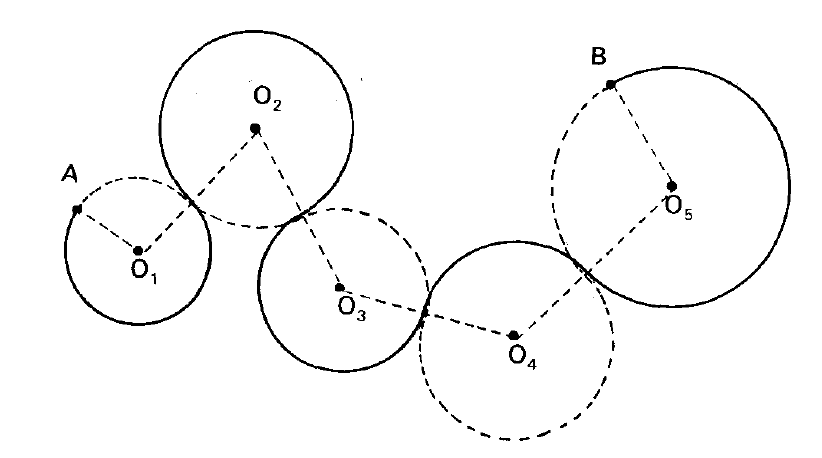
\includegraphics[width=0.8\textwidth]{article-image.png}
\caption{Imagem original que também compõe o enunciado do problema na Ref.,\cite{dolce-pompeo}; ela apresenta a configuração geométrica da curva $AB$, formada por arcos sucessivos de circunferências tangentes.}
\label{fig:geometric-configuration}
\end{figure}

\begin{proof}[\textbf{Solução}]

O exercício analisado propõe determinar o comprimento de uma curva formada por arcos sucessivos de circunferências tangentes, com ângulos e raios conhecidos. Como estabelecido no problema, são dados cinco centros, $O_1, O_2, O_3, O_4, O_5$, cada um associado a um ângulo central e a um raio específico. O objetivo é determinar o comprimento total da curva $AB$, construída a partir dos arcos externos dessas circunferências. Antes de prosseguir com a solução do problema, revisaremos uma definição útil referente a arcos de circunferência.


\begin{figure}[ht]
    \centering
    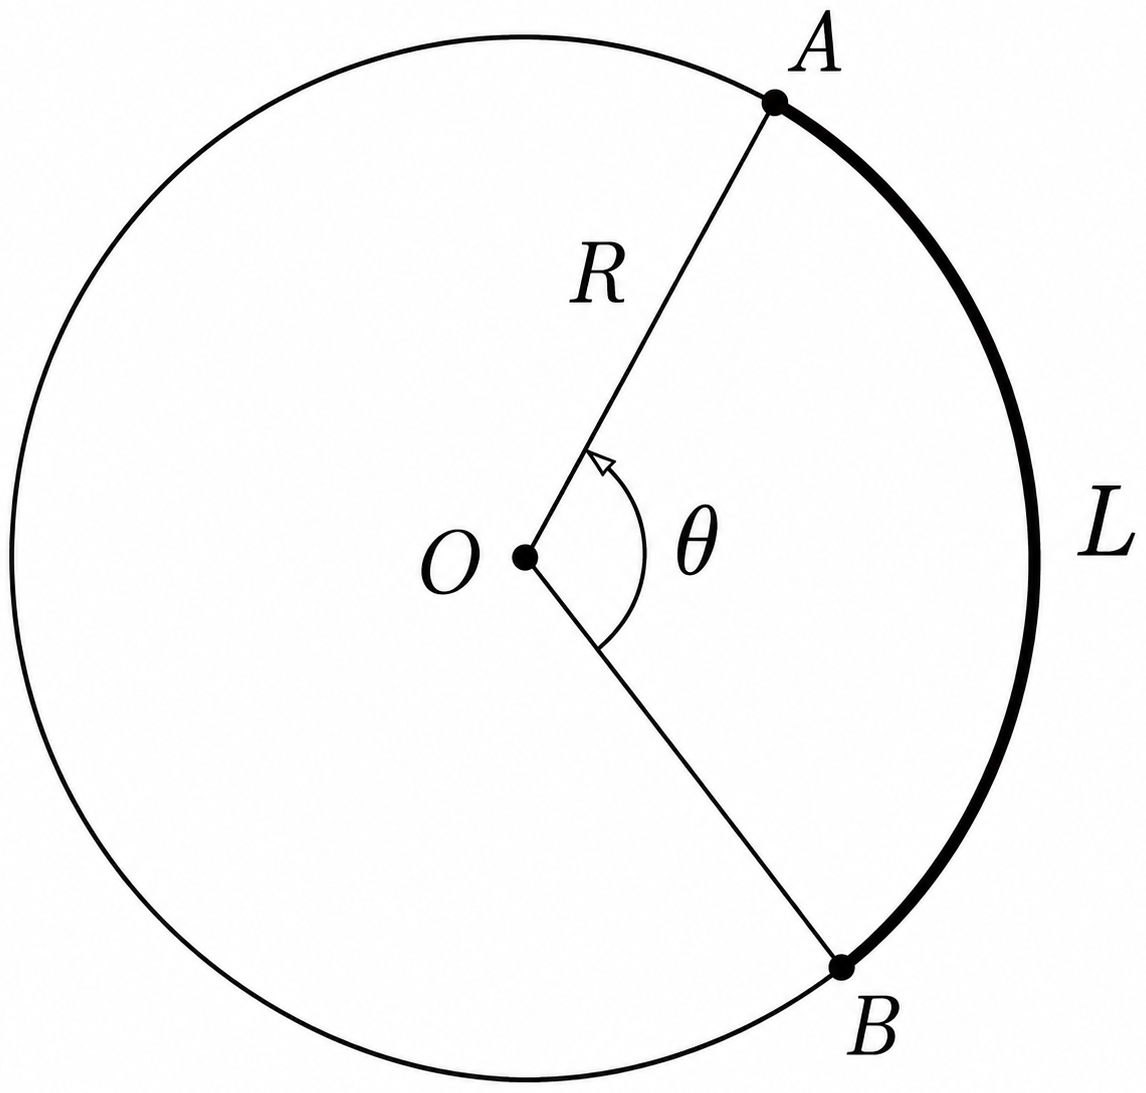
\includegraphics[width=0.4\textwidth]{circular_arc.png}
    \caption{Circunferência de raio $R$ e arco circular de comprimento $L$ subtendido por um ângulo $\theta$.}
    \label{circarc}
\end{figure}

Seguindo a Fig.,\ref{circarc}, vê-se imediatamente que o comprimento $L$ de um arco de circunferência de raio $R$ e ângulo central $\theta$, medido em radianos, decorre do fato de que a razão entre o comprimento do arco e o comprimento total da circunferência é igual à razão entre o ângulo central e o ângulo completo $2\pi$; matematicamente,

\be
\frac{L}{2\pi R} = \frac{\theta}{2\pi}.
\ee
Obtém-se $L = R\theta$. Se o mesmo ângulo for medido em graus e denotado por $\theta^{\text{(deg)}}$, então
\be
\theta = \frac{\pi}{180} \theta^{\text{(deg)}}.
\ee
Portanto, o comprimento de arco $L = R\theta$ também pode ser escrito como
\be
L = \frac{\pi}{180} R \theta^{\text{(deg)}}.
\label{eq1}
\ee
Os dados constituídos apenas pelos raios e pelos ângulos centrais não são suficientes para determinar o comprimento total, a menos que a configuração geométrica especifique qual arco de cada circunferência contribui para a curva. Para cada circunferência, o ângulo efetivo é ou o ângulo central dado, ou seu ângulo explementar. A configuração geométrica do problema impõe uma sutileza essencial: os arcos que formam a curva $AB$ não correspondem diretamente aos ângulos centrais dados, mas sim às porções externas das circunferências. Consequentemente, para cada circunferência, o ângulo relevante deve ser substituído por seu ângulo explementar $\alpha$, definido por
\be
\alpha_i = 2\pi - \theta_i.
\ee
Aplicando essa transformação às circunferências com centros em $O_1, O_2, O_3, O_5$ e mantendo o mesmo ângulo interno na circunferência com centro em $O_4$, obtém-se o seguinte conjunto de ângulos a utilizar no cálculo do comprimento total de $AB$: ${270^\circ, 288^\circ, 225^\circ, 120^\circ, 255^\circ}$. O comprimento total $L_{AB}$ da curva $AB$, formada pela cadeia de circunferências da Fig.,\ref{fig:geometric-configuration}, é então obtido pela soma de todos os arcos, considerando a Eq.,\eqref{eq1}. 
\be
L_{AB} = \frac{\pi}{180} \left(18 \cdot 270 + 35 \cdot 288 + 24 \cdot 225 + 36 \cdot 120 + 48 \cdot 255 \right).
\ee
Portanto, a resposta final para o comprimento total da curva $AB$ é
\be
L_{AB} = 205\pi.
\ee
Conclui-se, assim, a solução do problema.
\end{proof}

A Tabela~\ref{tab:data} resume os dados numéricos necessários para o cálculo do comprimento da curva $AB$. Para cada circunferência, a tabela apresenta o raio $R_i$, o ângulo $\theta_i$ dado no enunciado, o ângulo explementar correspondente $\alpha_i$, o ângulo efetivamente utilizado na fórmula do comprimento de arco e a contribuição resultante $L_i$. A quarta circunferência é o único caso em que o ângulo dado $\theta_i$ é utilizado diretamente; nos demais casos, os arcos relevantes são determinados pelos ângulos explementares $\alpha_i$.
\begin{table}[ht]
\centering
\caption{Dados utilizados no cálculo do comprimento de $AB$.}
\label{tab:data}
\begin{tabular}{c c c c c c}
\hline
Center & $R_i$ (cm) & $\theta_i$ & $\alpha_i$ & Angle used & $L_i$ \\
\hline
$O_1$ & $18$ & $90^\circ$  & $270^\circ$ & $\alpha_i$ & $27\pi$ \\
$O_2$ & $35$ & $72^\circ$  & $288^\circ$ & $\alpha_i$ & $56\pi$ \\
$O_3$ & $24$ & $135^\circ$ & $225^\circ$ & $\alpha_i$ & $30\pi$ \\
$O_4$ & $36$ & $120^\circ$ & $240^\circ$ & $\theta_i$ & $24\pi$ \\
$O_5$ & $48$ & $105^\circ$ & $255^\circ$ & $\alpha_i$ & $68\pi$ \\
\hline
\multicolumn{5}{l}{} & $205\pi$ \\
\hline
\end{tabular}
\end{table}


\section{Generalization}

O mesmo raciocínio se aplica a qualquer cadeia finita de $N$ circunferências tangentes, cujos arcos contribuintes são conhecidos a partir da configuração geométrica. Sejam as circunferências de raios $R_1, R_2,\ldots, R_N$, e sejam os ângulos centrais correspondentes, dados no enunciado, $\theta_1, \theta_2, \ldots, \theta_N$. Para cada circunferência, o arco que contribui para a curva $AB$ pode ser tanto o arco subtendido diretamente por $\theta_i$ quanto o arco subtendido por seu ângulo explementar
\be
\alpha_i = 2\pi-\theta_i,
\ee
quando os ângulos são medidos em radianos. Seja $\mathcal{I}*{\theta}$ o conjunto de índices para os quais o arco utilizado é o associado ao ângulo $\theta_i$, e seja $\mathcal{I}*{\alpha}$ o conjunto de índices para os quais o arco utilizado é o arco explementar associado a $\alpha_i$. Esses dois conjuntos formam uma partição do conjunto de índices:
\be
\mathcal{I}_{\theta}\cup \mathcal{I}_{\alpha}=\{1,2,\ldots,N\},
\qquad
\mathcal{I}_{\theta}\cap \mathcal{I}_{\alpha}=\varnothing.
\ee
Portanto, o comprimento total da curva $AB$ é dado pela expressão
\be
L_{AB} = \sum_{i\in\mathcal{I}_{\theta}} R_i\theta_i  + \sum_{i\in\mathcal{I}_{\alpha}} R_i\alpha_i.
\ee
Since $\alpha_i = 2 \pi - \theta_i$, this can also be written as
\be
L_{AB} = \sum_{i\in\mathcal{I}_{\theta}} R_i\theta_i + \sum_{i\in\mathcal{I}_{\alpha}} R_i(2\pi-\theta_i).
\ee
Se os ângulos forem dados em graus, então o ângulo efetivo utilizado para cada arco é
\be
\beta_i^{\mathrm{(deg)}} = 
\begin{cases}
\theta_i^{\mathrm{(deg)}}, & i\in\mathcal{I}_{\theta},\\[4pt] 360^\circ-\theta_i^{\mathrm{(deg)}}, & i\in\mathcal{I}_{\alpha}.
\end{cases}
\ee
Assim, o comprimento total torna-se
\be
L_{AB} = \frac{\pi}{180} \sum_{i=1}^{N} R_i\beta_i^{\mathrm{(deg)}}.
\ee
De forma equivalente,
\be
L_{AB} = \frac{\pi}{180} \left[ \sum_{i \in \mathcal{I}_{\theta}} R_i \theta_i^{\mathrm{(deg)}} + \sum_{i\in\mathcal{I}_{\alpha}}R_i \left(360^\circ-\theta_i^{\mathrm{(deg)}} \right) \right].
\ee
Para o problema particular analisado na seção anterior deste trabalho
\be
N=5, \qquad \mathcal{I}_{\theta}=\{4\}, \qquad \mathcal{I}_{\alpha}=\{1,2,3,5\}.
\ee

\section{Conclusão}

O problema discutido neste trabalho ilustra como uma questão elementar de geometria plana pode levar a uma generalização. Partindo de uma configuração específica de circunferências tangentes, mostramos que o comprimento da curva $AB$ é obtido ao identificar, para cada circunferência, o arco efetivo que a contribui. Esse ponto é essencial: os dados numéricos isoladamente, constituídos pelos raios e pelos ângulos centrais, não determinam a resposta, a menos que a configuração geométrica especifique se o arco relevante está associado ao ângulo central dado ou ao seu ângulo explementar.

\begin{thebibliography}{9}

\bibitem{dolce-pompeo}
DOLCE, Osvaldo; POMPEO, José Nicolau. \textit{Fundamentos de Matemática Elementar: Geometria Plana}. Vol.~9, 7th ed. São Paulo: Atual Editora, 1993.

\end{thebibliography}

\end{document}